\documentclass[tikz, border=10pt]{standalone}
\usepackage{pgfplots}
\pgfplotsset{compat=1.18}

\begin{document}
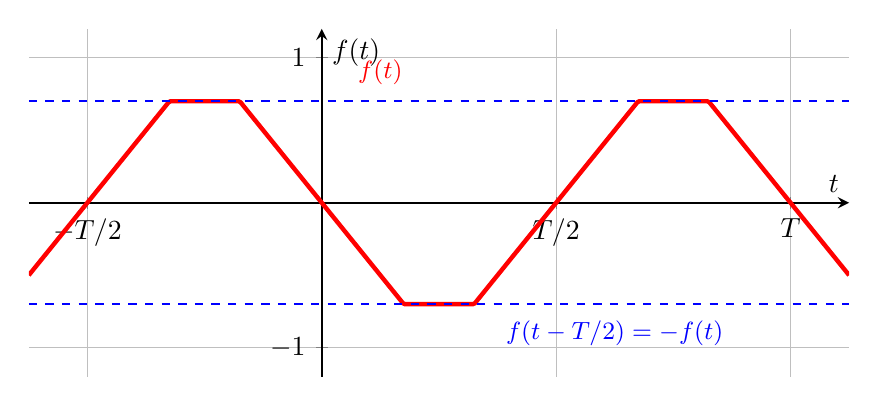
\begin{tikzpicture}
    \begin{axis}[
        width=12cm, height=6cm,
        axis lines=middle,
        xlabel={$t$}, ylabel={$f(t)$},
        ymin=-1.2, ymax=1.2,
        xmin=-2.5, xmax=4.5,
        xtick={-2, 0, 2, 4},
        xticklabels={$-T/2$, 0, $T/2$, $T$},
        grid=both,
        samples=400,
        domain=-2.5:4.5,
        thick
    ]
        % Odd + HWS: Clipped triangle wave
        % Triangle area: 1 - abs(x) for -1 < x < 1 (T=2)
        % For HWS compliance: shifted version must be negative
        % f(x) = clipped triangle: max(-0.7, min(0.7, triangle))
        % Period T=4, T/2=2
        \addplot[red, ultra thick] {max(-0.7, min(0.7, 
            ( (mod(x+2, 4) < 2) ? (1 - abs(mod(x+2, 4) - 1)) : -(1 - abs(mod(x+2, 4) - 3)) )
        ))};
        
        \node[red] at (axis cs:0.5, 0.9) {\small $f(t)$};
        \node[blue] at (axis cs:2.5, -0.9) {\small $f(t-T/2) = -f(t)$};
        
        \draw[dashed, blue] (axis cs:-2.5, 0.7) -- (axis cs:4.5, 0.7);
        \draw[dashed, blue] (axis cs:-2.5, -0.7) -- (axis cs:4.5, -0.7);
    \end{axis}
\end{tikzpicture}
\end{document}
